\section{Title}
\newrefsegment

%---------------------------------------------------------------------------------
\section*{Quality Assurance}
\begin{tabular}{@{}p{27mm}@{}p{0mm}p{\textwidth-52mm-48pt}p{15mm}p{10mm}}
\textbf{Date} & \textbf{:} &  26 July 2018 \\ 
\textbf{Author} & \textbf{:} &  Jaco Stout & \textbf{Initials:} & \ldots \\
\textbf{Review} & \textbf{:} &  Erik de Goede & \textbf{Initials:} & \ldots 
\end{tabular}

%---------------------------------------------------------------------------------
\section*{Version information}
\begin{tabular}{@{}p{23mm}@{}p{0mm}p{\textwidth-23mm-30pt}}
\textbf{Date of study}& \textbf{:} & 26 July 2018 \\
\textbf{Executable}   & \textbf{:} & Deltares, Delft3D FM 2018.03 (1.4.6.40270), July 30 2018 \\
\textbf{Location}     & \textbf{:} & \url{https://repos.deltares.nl/repos/DSCTestbench/trunk/cases/e105_dflowfm_drtc/f01_general/c077_gate_lowering_closed_door} \\ 
\textbf{SVN revision} & \textbf{:} & -
\end{tabular}

%---------------------------------------------------------------------------------
\section*{Purpose}

This test is meant to test the BMI-compliancy of D-Flow FM and D-RTC, exchanging the position (movement) of a \menu{General Structure} or \menu{Gate}. This test is one in a serie of 4 tests for the \menu{General Structure} (c070 -- c073) and 4 tests for the \menu{Gate} (c074 -- c077).

%---------------------------------------------------------------------------------
\section*{Linked claims}
Closing the doors in horizontal direction of a general structure will close the structure and after a while there is overtopping. 
Opening the doors in horizontal direction will open the structure and after a while there is no overtopping any more.

%---------------------------------------------------------------------------------
\section*{Approach}

This test is a clone of the stand-alone D-Flow FM test (chapter e02). In the stand-alone test a time series (for the movement of the structure) is specified with the Gate or General Structure itself. In this test this timeseries has been moved to a time-rule in D-RTC, which controls that same structure. The simulated movement of the structure should therefore be identical to that of the stand-alone test (e02).

%---------------------------------------------------------------------------------
\section*{Conclusion} 
The doors of a general structure are closing in horizontal direction correctly.

%---------------------------------------------------------------------------------
\section*{Model description}

The (hydrodynamic) model is identical to the corresponding stand-alone D-Flow FM testcases for gates and general structures (e02). The model is based on the model used in some stand-alone D-Flow FM testcases, testing morphology and boundary conditions (\url{e02_dflowfm/f22_morphology_2D/c23_boundary_condition_icond3}).

\begin{figure}[H]
    \centering
    \includegraphics*[width=0.85\textwidth]{figures/model_outline.png}
    \caption{layout of the model: a schematic model of the \menu{RijnMaasMonding (RMM)}}
\end{figure}

The Maeslantkering in this model - not in it's true dimensions - is controlled by D-RTC: \menu{Time rules} for:

\begin{itemize}
  \item \menu{Lower edge level} exchanged to D-Flow FM as \menu{gateheight}
  \item \menu{Opening width} exchanged to D-Flow FM as \menu{door\_opening\_width}
  \item \menu{Sill level} exchanged to D-Flow FM as \menu{levelcenter}
\end{itemize}

Below are the input time series.

\begin{tabular}{@{}p{1.5in}|p{1.2in}|p{1.8in}|p{\textwidth-4.5in-12pt}@{}}
\textbf{Date Time} & \textbf{gateheight [m]} & \textbf{door\_opening\_width [m]} & \textbf{levelcenter [m]} \\ [1ex] \hline \STRUT
\ 2007-01-01  00:00:00 & -16.5 & 1000.0 & -16.5 \\
\ 2007-01-04  11:20:00 & -16.5 & 1000.0 & -16.5 \\
\ 2007-01-07  22:40:00 & -16.5 &    0.0 & -16.5 \\
\ 2007-01-14  21:20:00 & -16.5 &    0.0 & -16.5 \\
\ 2007-01-18  08:40:00 & -16.5 & 1000.0 & -16.5 \\
\ 2007-01-21  20:00:00 & -16.5 & 1000.0 & -16.5 \\
\end{tabular}

%---------------------------------------------------------------------------------
\section*{Results}

The position (movement) of the structure is written to the \ext{*.nc}-file.

%---------------------------------------------------------------------------------
\section*{Analysis of results}

The resulting movement of the structure must be the same as the input timeseries of the corresponding \menu{Time rule}.

With the start of closing the doors at 2007-01-04 11:20:00 there is a small disturbance in the water level, see \autoref{fig:e105f01c071_closing_disturbance}. 
When the doors are closed, the water level will increase at the river side of the structure (upstream side). 
At 2007-01-10 20:00:00 the water level will reach the level of \SI{5.5}{\metre} which is exactly the \textsl{gate upper edge level} (5.5 = -16.5 + 22; i.e.\ level center + door height), and water will flow over the doors.
So after a while there will be a discharge of \SI{1500}{\cubic\metre\per\second} over the doors, so called over topping.
When the doors are start moving to open at 2007-01-14 21:20:00 a translation wave will occur, because the head difference between the downstream- and upstream side of the structure is \SI{6.573}{\metre}.
At 2007-01-15 08:30:00 the upstream side water level reach again the value of
\SI{5.5}{\metre}, so the discharge due to overtopping is stopped now, and again a disturbance is seen, see \autoref{fig:e105f01c071_whole_time_series}.
From now on there is only a flow in between the doors and the waterbody will return to a stationary state.

\begin{figure}[H]
\begin{center}
	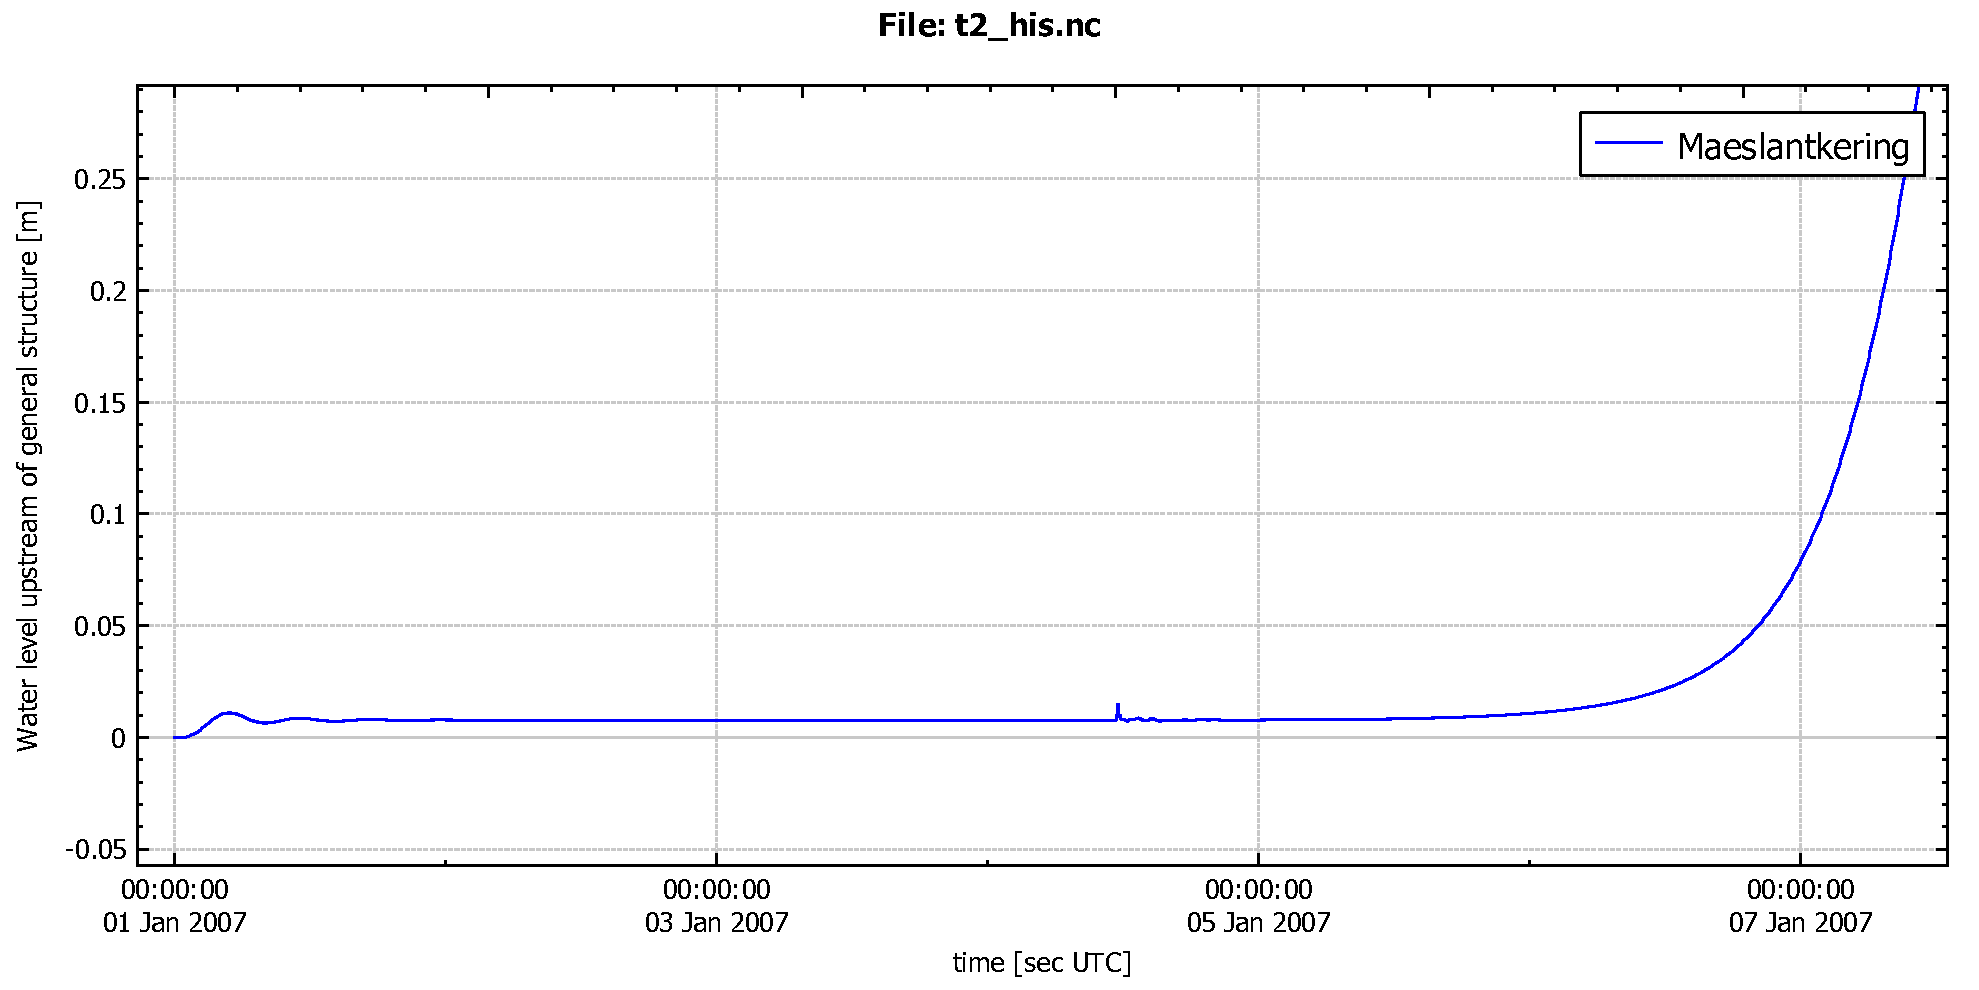
\includegraphics[width=0.9\textwidth]{figures/waterlevel_at_closing.pdf}
	\caption{Disturbation of the upstream water level when the doors start to close.\label{fig:e105f01c071_closing_disturbance}}
\end{center}
\end{figure}

\begin{figure}[H]
	\begin{center}
		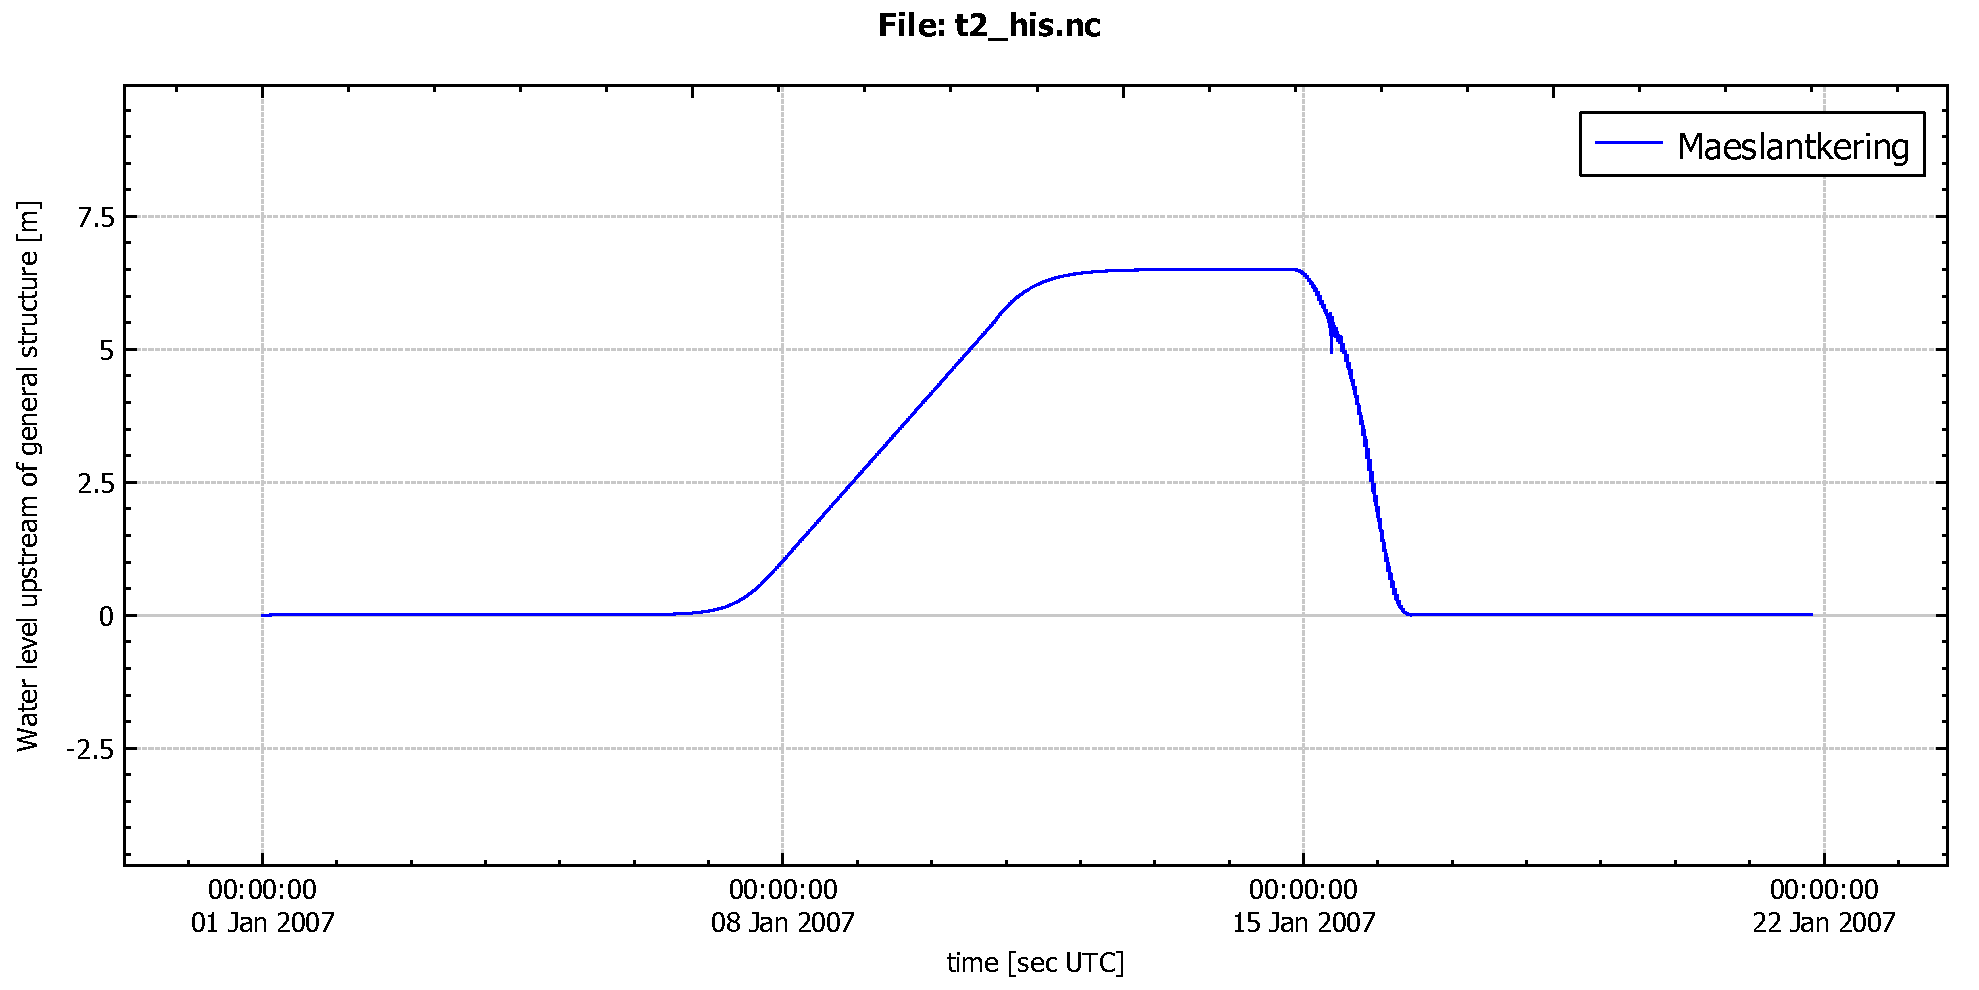
\includegraphics[width=0.9\textwidth]{figures/waterlevel_upstream.pdf}
		\caption{Complete time series of the upstream water level.\label{fig:e105f01c071_whole_time_series}}
	\end{center}
\end{figure}
%---------------------------------------------------------------------------------
\printrefsegment
